\documentclass{article}
\usepackage[french]{babel}
\usepackage[T1]{fontenc}
\usepackage[letterpaper,top=2cm,bottom=2cm,left=3cm,right=3cm,marginparwidth=1.75cm]{geometry}
\usepackage{wrapfig}
\usepackage{float}
\usepackage{graphicx}
\usepackage{setspace}
\usepackage{blindtext}
\usepackage{amsmath}
\usepackage{amssymb}
\usepackage{array}
\usepackage{booktabs}
\usepackage[colorlinks=true, allcolors=black]{hyperref}

\title{\textbf{\textsf{\Huge{Rapport de Projet}\\\huge {HAI405I}}}}
\author{SAVY Lisa, GILLES Eric, GALLERNE Romain, NAVEL Morgan\\
{\Large Groupe S}\\
\url{https://github.com/eric-gilles/Projet_Prog}\\
  L2 informatique\\
  Faculté des Sciences, Université de Montpellier}
\date{{\Large \textsf{\today}}}
\begin{document}
    \maketitle
    \vspace{0.5cm}
    \begin{figure}[h]
        \centering
        
\includegraphics[width=10cm]{images/Logo-QuiEstce.png}
    \end{figure}
    
    \begin{abstract}
        \centering
        {\textsl{Jeu Qui Est-Ce ? avec un générateur et un mode double personnage \\
        réalisé par le Groupe S de L2 Informatique}}
    \end{abstract}
    
    \pagebreak
    
    \tableofcontents
    
    \pagebreak
    
    \section{Technologies utilisées  et organisation}
        \vspace{0.5cm}
        {\large Le projet consiste en la réalisation d’une réplique du jeu \textsf{Qui est-ce ?}, ainsi que d’un générateur de fichiers JSON, qui pourront par la suite être utilisés dans le jeu.\\
        Il faudra également ajouter une extension parmi les choix suivants :}
        
        \begin{itemize}
            \item Jouer contre l’ordinateur
            \item Jouer à deux
            \item Jouer avec deux personnages cachés
        \end{itemize}
        
        \subsection{Choix du langage}
            Pour notre projet, nous avons fait le choix d’utiliser JavaScript. Plusieurs raisons nous ont poussé vers ce langage :
            \begin{itemize}
                \item
                    Dans ce projet, nous allons manipuler un fichier JSON (JavaScript Object Notation) et le JavaScript est donc un langage particulièrement adapté pour cela.
                \item
                    Concernant la partie graphique, nous avons fait le choix de nous orienter vers une application web et ce grâce à JavaScript. En effet, on peut modidier des objets dans le DOM d’un site web et même utiliser des bibliothèques graphiques (par exemple D3JS).
                \item 
                    Il existe dans JavaScript beaucoup de bibliothèques particulièrement puissantes, notamment JQuery qui nous sera très utile pour accéder aux différents éléments de la page.
            \end{itemize}

        \subsection{Organisation du travail}
            \subsubsection{Jeu et Extension}
                \begin{itemize}
                    \item Morgan s’est occupé de l’affichage et l’initialisation des questions.
                    \item Lisa s’est occupé du CSS et du choix aléatoire du personnage.
                    \item Morgan et Lisa se sont, en parallèle de la construction des questions, occupés de l’extension \textsf{Mode Double Personnage}.
                    \item Romain a développé les fonctions liées au mode \textsf{Facile} et l’affichage des personnages ainsi que le retournement des images et le traitement des questions.
                    \item  Éric a développé les fonctions liées à la sauvegarde, au chargement du jeu en cours et le test de choix de personnage.
                \end{itemize}

            \subsubsection{Générateur}
                \begin{itemize}
                    \item Morgan et Lisa ont développé les fonctions liées aux attributs.
                    \item Romain a développé les fonctions liées la création de personnages.
                    \item Éric a développé les fonctions d'import d’images et la conversion des objets Javascript en un fichier JSON.
                \end{itemize}
            
            \subsubsection{Rapport}
                \begin{itemize}
                    \item Morgan s'est occupé de rédiger la partie sur l'extension.
                    \item Lisa s'est occupé de rédiger la partie sur le générateur et du rendu final du rapport.
                    \item Romain s'est occupé de rédiger la partie sur le jeu principal.
                    \item Éric s'est occupé de rédiger l'introduction et la conclusion.
                \end{itemize}
                
            \subsubsection{Rythme de travail, mode de fonctionnement}
                Travail pendant 3h au moins par semaine pendant les périodes prévus dans l’emploi du temps plus les week-end et toutes les après-midi des vacances.
    \pagebreak
    
    \section{Jeu principal : Permettre à l'utilisateur de jouer}
        \vspace{0.5cm}
        Afin de permettre à l'utilisateur de jouer à un jeu fidèle au jeu d'origine, nous avons incorporé de nombreuses fonctionnalités à notre application, nous allons les détailler ici.
        \begin{figure}[h]
            \centering
            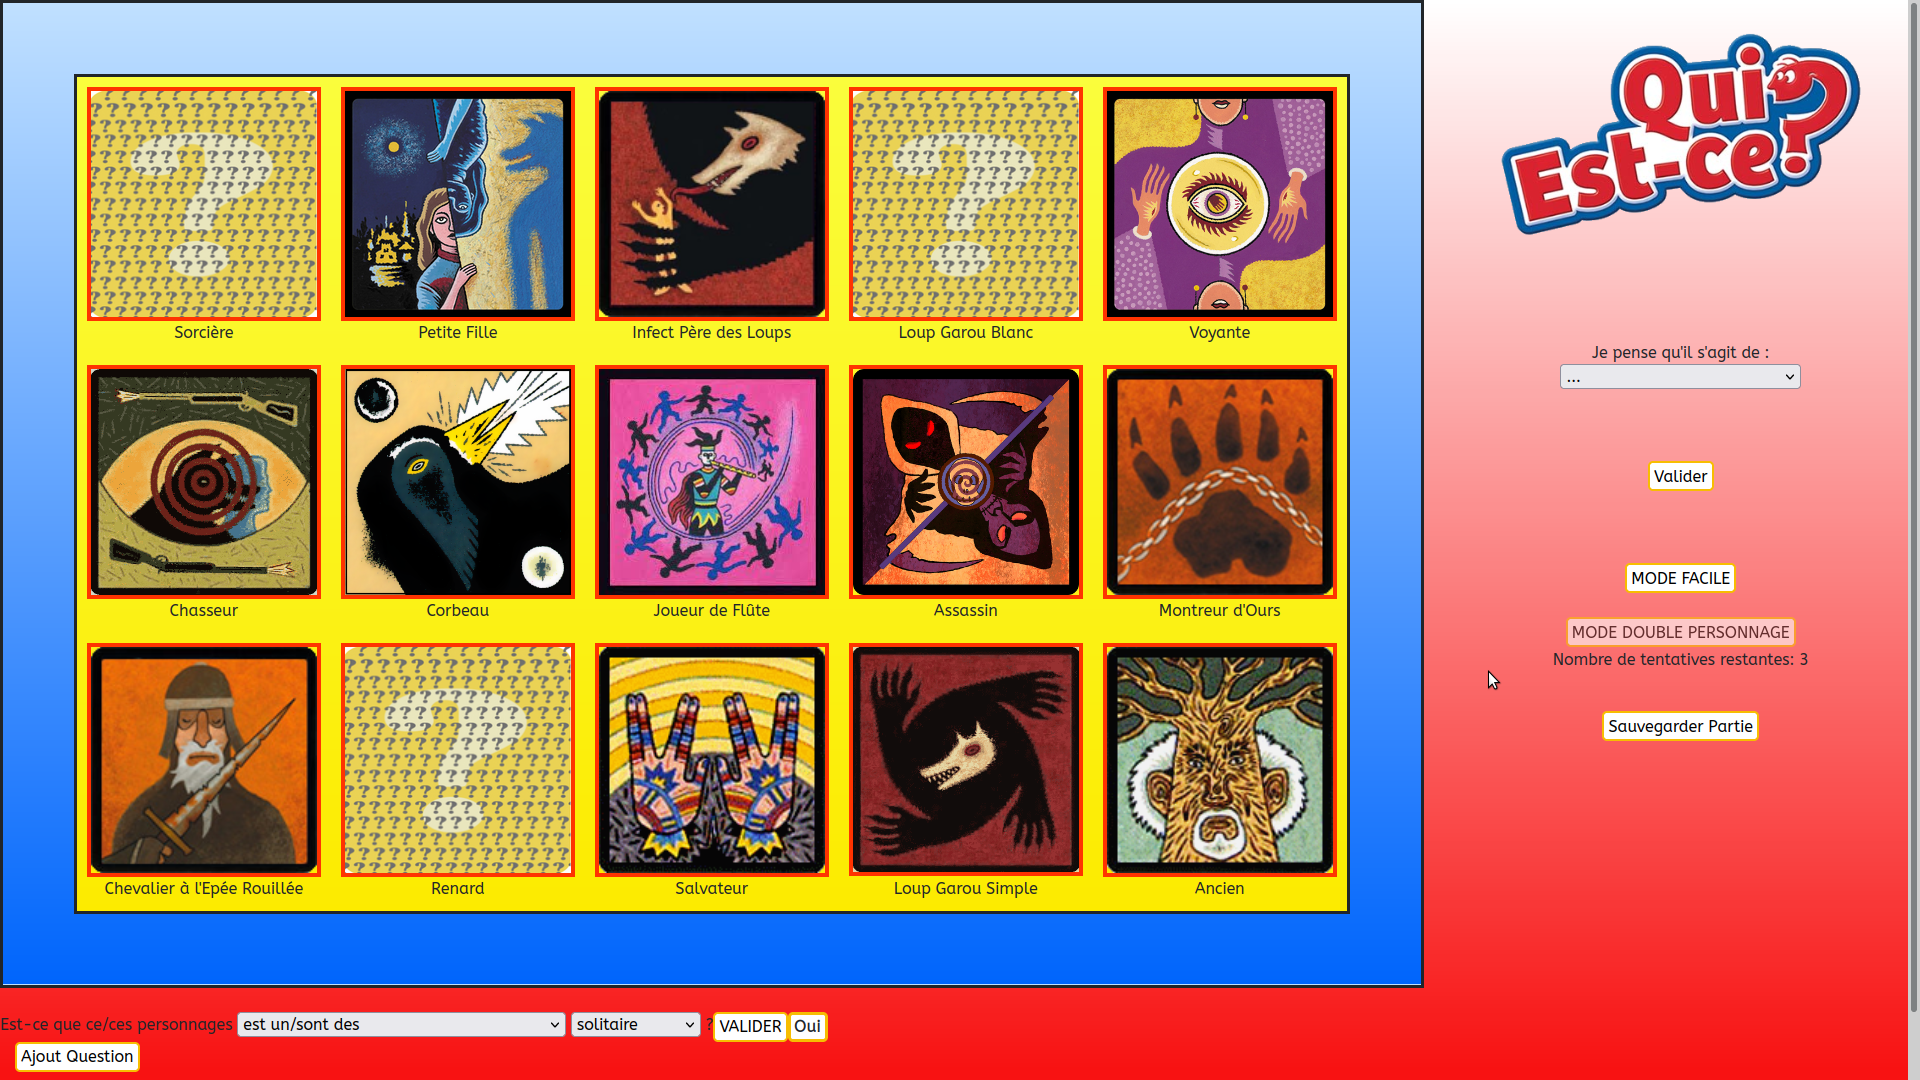
\includegraphics[width=13.5cm]{images/CaptureJeuQuiEstCe.png}
            \caption{Rendu du Jeu \textsf{Qui est-ce?}}
            \textit{Capture d'écran de la page de jeu principal en cours de partie.}
        \end{figure}
        
        \subsection{Fonctionalités de l'application}
            Le point le plus important d'un logiciel d'un point de vue utilisateur est bien sûr les fonctionalités offertes par le dit logiciel (cf. \textsc{Figure 1}). Nous avons donc mis l'accent sur les diverses possibilités que notre application offriraient au joueur, à commencer par différents mode de jeu.
            
            \subsubsection{Mode de jeu Normal}
  		        Tout d'abord, dès son arrivée sur l'application, l'utilisateur doit en premier lieu importer un fichier JSON de son choix, compatible avec le jeu.\\
  		        Le formalisme de ces fichiers et leur générateur seront détaillés dans d'autres parties.\\
  		        Une fois le fichier choisi par l'utilisateur, il suffit à celui-ci de presser le bouton \textsc{Importer} (cf. \textsc{Figure 2}). Le logiciel traite alors le fichier JSON et affiche de lui-même la grille de jeu. Il pré-génère également les questions qui pourront être posées en fonction des attributs dans le fichier.\\
  		        Afin d'empêcher toute fausse manipulation, nous retirons le bouton d'importation lorsque tout a été convenablement généré.\\
  		        \begin{figure}[h]
          			\centering
          		    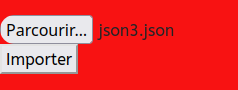
\includegraphics[width=6cm]{images/BoutonImport.png}
          			\caption{Bouton d'import du fichier JSON}
          			\textit{Situé en bas à gauche de la page, il permet de choisir un fichier JSON et déclenche automatiquement toutes les fonctions de traitements afin d'afficher la grille de jeu.}
		        \end{figure}
		        \pagebreak
  	            \par
  	                Une fois le fichier JSON importé, le jeu se met en place. La grille de jeu est affichée et les questions sont pré-chargées. L'utilisateur peut alors poser diverses questions dépendantes des attributs des personnages. Le joueur peut demander la valeur précise de chaque attributs, par exemple il pourra demander\\
  	                \textit{Est-ce que ce/ces personnages a/ont les cheveux blonds ?} (L'écriture au pluriel prévoyant plusieurs personnages est utile pour le mode \textsf{Double Personnage}, nous y reviendrons par la suite).\\
  	                Une fois la question validée, l'application répond par "\textsc{Oui}" ou "\textsc{Non}", c'est alors à l'utilisateur de déduire les personnages à retourner.\\
  	            	Lorsque l'utilisateur le souhaite, il peut retourner une case (cf. \textsc{Figure 3}). L'opération est évidemment réversible.\\
  		            Cette action n'a aucun effet sur le fonctionnement du programme et est purement dédiée à l'utilisateur afin qu'il puisse trier les personnages librement.\\
  		        \begin{figure}[h]
          			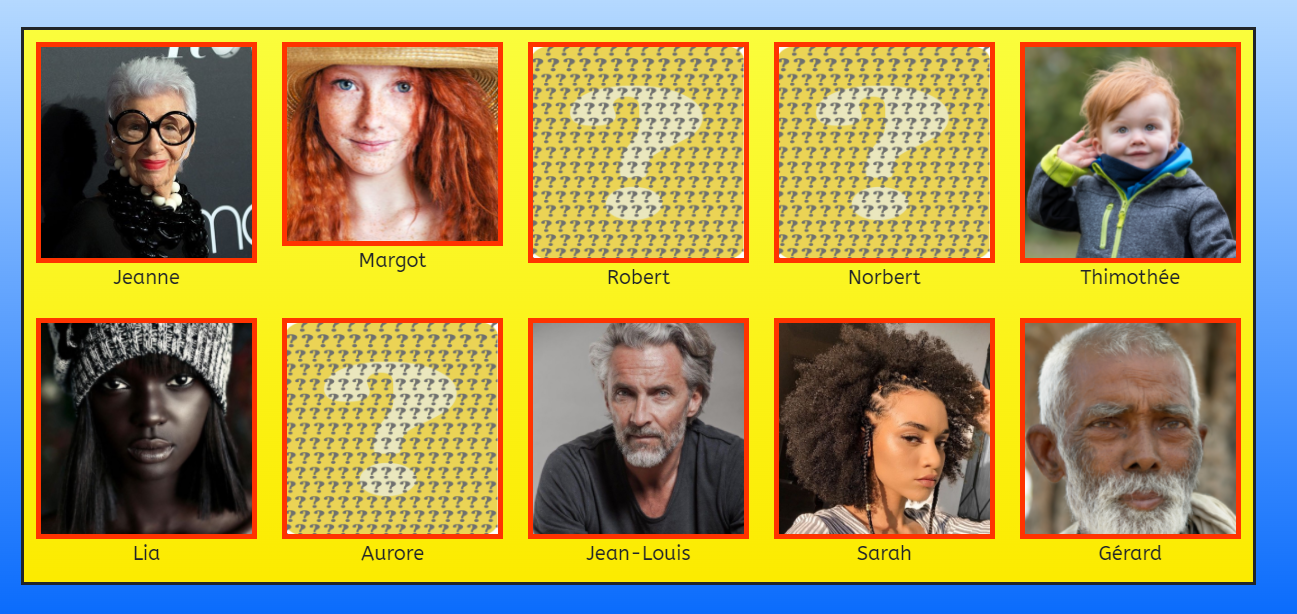
\includegraphics[width=11cm]{images/Retournement.PNG}
          			\centering
          			\caption{Face retournée des personnages}
          			\textit{La carte se retourne pour laisser place à un point d'intérogation.}
        		\end{figure}
        	    \par
        		Quand le joueur pense avoir une idée de la réponse, il peut formuler une hypothèse dans le menu de sélection des réponses.\\
        		Le joueur doit alors choisir le personnage qu'il pense être le bon et presser le bouton \textsc{Valider} (cf. \textsc{Figure 4}). Si le joueur aboutit à la bonne réponse, alors une fenêtre est affichée pour le féliciter et le jeu se relance automatiquement après fermeture de la dite fenêtre.\\
        		Dans le cas contraire, le nombre d'essais restants (3 dans le mode \textsf{Normal}) est décrémenté. Si celui-ci atteint 0, c'est perdu.\\
        		\begin{figure}[h]
          			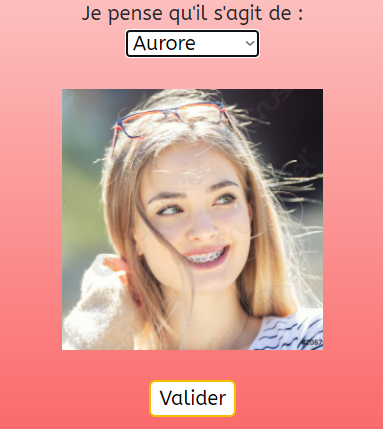
\includegraphics[width=5cm]{images/Choix.PNG}
          			\centering
          			\caption{Menu de séléction d'une réponse}
          			\textit{Ici, le joueur pense qu'Aurore est la bonne réponse, son image \\s'affiche alors au dessous afin d'éviter toute erreur avant la validation}
        		\end{figure}
        		\par
        		\pagebreak
        		L'une des dernières fonctionalités principales de notre application est la sauvegarde de la partie. Si l'utilisateur ferme la page durant la partie, à sa prochaine visite, il lui sera possible de recharger en l'état la partie quittée précedemment. Les personnages retournés le seront ainsi que le nombre de tentatives et le mode de jeu. Nous utilisons ici la sauvegarde locale des pages web afin de gérer cette sauvegarde.
        		
		    \subsubsection{Mode Facile}
		        Juste en-dessous du menu de sélection de la réponse, le joueur peut activer à tout moment de la partie le mode \textsf{Facile}, nous allons détailler les changements qu'entraine l'activation du mode \textsf{Facile} dans le déroulement de la partie.\\
		    \par
		        L'impact le plus notable du mode \textsf{Facile} sur le fonctionnement du jeu est l'apparition d'un bouton \textsc{Estimer} à côté du bouton de validation des questions. De fait, ce bouton permet, après formulation d'une question, de retourner au joueur le nombre de personnages que cette question éliminera, c'est-à-dire le nombre de cases qui pourront être retournées. Cette estimation prend évidemment en compte la logique des questions multiples énoncée ci-après.\\
	        	Un autre changement notable est le retournement automatique des cases. En effet, dès l'appui du bouton \textsc{Valider}, le programme retournera alors de lui-même l'entièreté des cases qui doivent l'être, facilitant grandement la tâche du joueur. À noter qu'il n'est pas difficile de démontrer qu'on peut aboutir à un unique personnage non-retourné en un nombre fini de questions.\\
		        Enfin, le nombre de tentatives restantes augmente de 2, totalisant 5 tentatives pour laisser plus de possibilités.\\
		        \par
		        L'activation du mode \textsf{Facile} empêche celle du mode \textsf{Double Personnage} (notre extension) que nous avons considéré comme étant un mode \textsf{Difficile}, il n'est donc pas compatible avec le mode dont nous parlons.
		
  		\subsection{Le format du fichier JSON}
            Le format du fichier JSON a été décidé de façon à respecter le langage naturel. Nous avons donc opté pour un format fixe de question .\\
            \begin{figure}[h]
                \centering
                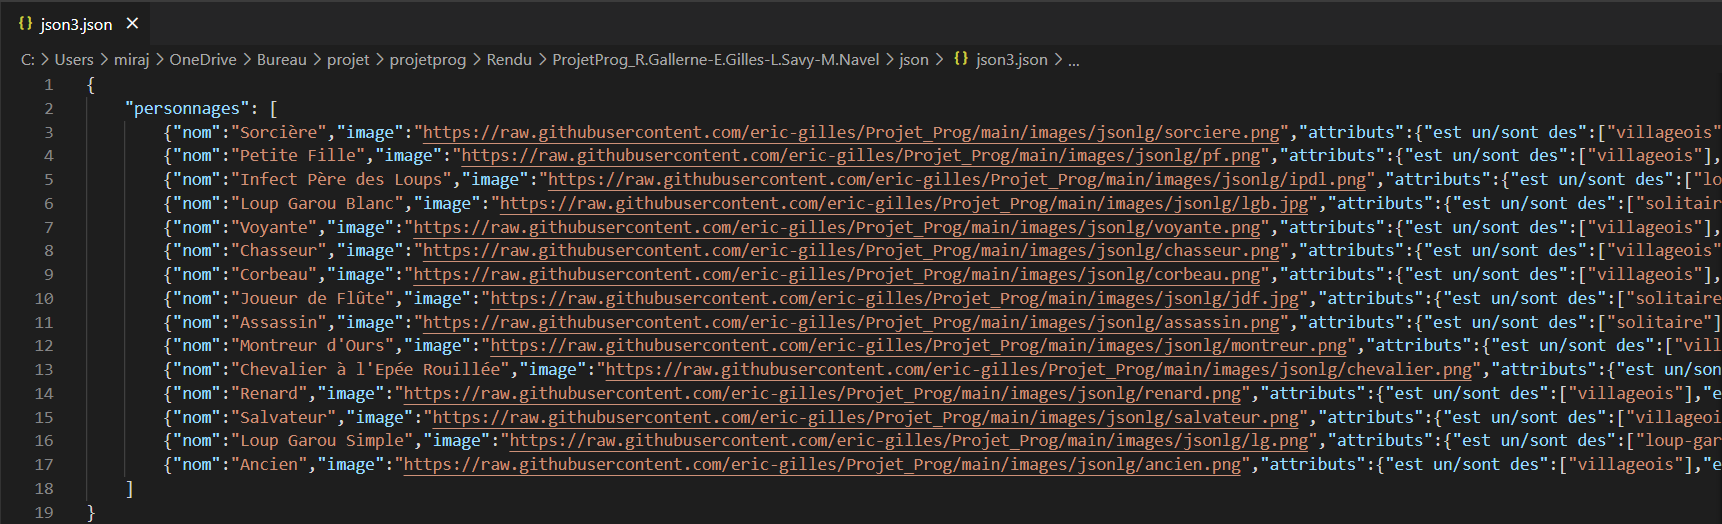
\includegraphics[width=15.5cm]{images/formatjson.png}
                \caption{Exemple d'un fichier JSON}
            \end{figure}\\
            Comme on peut le voir sur la \textsc{Figure 5}, le fichier JSON contient un seul attribut : "\texttt{personnages}", ayant pour valeur un tableau de dictionnaires où chaque dictionnaire représente un personnage de la grille.
            Chaque dictionnaire de personnage possède trois attributs :
            \begin{itemize}
                \item "\texttt{nom}", ayant pour valeur le nom du personnage,
                \item "\texttt{image}", ayant pour valeur le lien de l'image et
                \item "\texttt{attributs}", ayant pour valeur un dictionnaire représentant les attributs du personnage et leurs valeurs.
            \end{itemize}
  		
		\subsection{Formatage des requêtes}
		    Nous avons fait le choix de nous rapprocher au maximum du langage naturel afin de permettre, même aux utilisateurs les moins aguerri, d'utiliser sans soucis notre logiciel.\\
		    \par
		    Pour cela, nous avons organisé nos données de façon à ce que les questions puissent s'assembler en langage naturel. Nous avons donc, sur la page, le début de la question déjà affichée lorsque la cette dernière est créée : \textit{Est-ce que ce/ces personnages}.\\
		    Ensuite, c'est à l'utilisateur de choisir parmi la liste des attributs celui qu'il souhaite utiliser.\\
		    L'ensemble des attributs sont ainsi noté ici, mais encore une fois sous la forme du langage naturel, on ne notera donc pas l'attribut \textsf{cheveux} mais bien \textit{a/ont les cheveux}. On précisera ensuite la valeur de cet attribut, ici, par exemple, \textit{blonds} afin de former la question \textit{Est-ce que ce/ces personnages a/ont les cheveux blonds ?} (cf. \textsc{Figure 6}).
    		\begin{figure}[h]
      			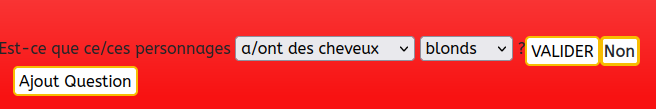
\includegraphics[width=12cm]{images/Questions.PNG}
      			\centering
      			\caption{Séléction d'une question}
      			\textit{On voit ici que les noms d'attributs et leurs valeurs s'agencent afin de former une question correcte en langue française. Nous avons cependant dû prévoir la présence du pluriel pour l'extension double personnage que nous détaillerons dans la Partie 4.}
    		\end{figure}
		
  		\subsection{Structures de données utilisées}
  		    Notre programme étant réalisé en JavaScript, donc en format Web, nous sommes amenés à manipuler à de très nombreuses reprises des objets au format DOM pour l'affichage. Concernant la logique, nous utilisons majoritairement des variables et objets JavaScript.
  		    
  		    \subsubsection{Données web, modification du DOM}
  		        \par Le DOM (Document Object Model) est le format des objets présents sur la page Web. Celui-ci est généré directement par le navigateur dépendamment du code HTML fourni.\\
  		        Afin de gérer les différents objets de la page tels que la liste des questions, l'affichage des cases (retournées ou non), l'affichage du personnage séléctionné ou encore la désactivation des boutons, nous sommes sans cesse contraints de modifier les objets du document. C'est pour cela que, pour la majorité de ces données, nous n'avons nullement besoin de les stocker dans un format de données autre puisque nous les positionnons directement dans le DOM là où elles sont à la fois disponibles pour l'utilisateur mais également consultables et modifiables à tout moment par le programme comme des variables.\\
  		        \par C'est donc dans ce format que nous chargeons les données importantes telles que les images des personnages ou bien la liste des attributs et leur valeurs possibles directement depuis le fichier JSON importé.\\
  		        D'autres éléments de la page, comme les questions, sont référencés par leur attributs "\texttt{id}" dans le DOM. Les valeurs de ces attributs sont générées par des compteurs globaux comme \texttt{NombreQuestions} ou \texttt{EssaisRestants}. Toutes ces données, qui doivent être accessible partout et à tout moment, sont référencées globalement. Par exemple, pour l'attribut de la seconde question, on lui attribuera l'id "attribut"+NombreQuestions, ce qui donnera "attribut1" (1 car nous commençons le compte à 0 et non à 1).
  		    \pagebreak
  		    \subsubsection{Données utilitaires, du JSON au programme}
  		        Nous devons récupérer toutes les données du fichier JSON afin de les transformer en un format Objet.\\
  		        C'est ici que s'illustre tout particulièrement le choix de notre langage, le JavaScript. Effectivement, le JavaScript permet un traitement très complet du format JSON, le transformant aisément en objet JavaScript (JSObject) dont le format est le même. Ainsi, dès l'import du fichier JSON, nous l'extrayons dans un objet JavaScript global que nous utiliserons par la suite dans tout le programme afin à ne pas avoir à récupérer le fichier à chaque retouche.\\
  		        Au passage, nous y choisissons aléatoirement un élément qui deviendra la réponse attendue, le personnage à deviner. Celui-ci sera stocké au format JSObject dans une variable globale à part.
		
  		    \subsection{Traitements des requêtes}
  		        On distingue dans notre jeu trois types de requêtes différentes pouvant être formulées par l'utilisateur :
  		        \begin{itemize}
  		            \item les requêtes de questions et leurs variantes.
  		            \item les requêtes d'estimation.
  		            \item les requêtes d'hypothèses.
  		        \end{itemize}
		    
		        \subsubsection{Requêtes des questions}
                    \par Afin de permettre de plus amples possibilités de jeu, il est possible ici d'ajouter d'autres questions, liées par une logique booléenne. Avec un maximum de 16 questions, le programme aboutit a une seule réponse générée logiquement avec une priorité pour la dernière question.\\
                    Par exemple, posons \texttt{c} le connecteur "\textsc{et}" ou "\textsc{ou}", et " \texttt{1}", " \texttt{2}", ..." \texttt{16}" les 16 questions possibles. La logique sera traitée par le programme de la manière suivant :  \texttt{(((1 c 2) c 3) c 4 ...) c 16}. Le joueur formule une ou des questions dans la zone appropriée et presse le bouton \textsc{Valider}, la logique des questions s'enclenche alors afin d'aboutir à une réponse unique.\\
                    \par Pour permettre cela, nous devons d'abord déterminer la réponse individuelle de chaque question. Dans une fonction dédiée appelée \texttt{TraitementUneQuestion()} prennant en paramètres l'attribut ainsi que sa valeur, par exemple "\textit{a/ont les cheveux}" et "\textit{blonds}". On vérifie alors que, pour la bonne réponse, pour rappel, référencé dans une variable globale au format JSObject, à l'index passé en paramètres, ici, "\textit{a/ont les cheveux}", on trouve bien la même valeur, ici, "\textit{blonds}". Si c'est le cas alors on retourne la valeur booléenne \texttt{True}, sinon \texttt{False}.\\\\
                    Enfin, une fonction à part appellé \texttt{TraitementQuestion()} s'occupe d'assembler la réponse de toutes ces questions d'après la logique formulée ci-dessus. \\
                    On aboutit donc à une réponse finale qui sera affichée à l'utilisateur : 
                    \begin{itemize}
                        \item Oui, si le résultat est \texttt{True}.
                        \item Non, si celui-ci est \texttt{False}.
                    \end{itemize}
		
		        \pagebreak
		        \subsubsection{Requêtes d'estimation et retournement automatique}
		            \par Les requêtes d'estimations sont une variante des requêtes de questions puisqu'elles utilisent exactement la même logique, à ceci prêt que nous ne cherchons pas simplement à aboutir à une réponse mais bien à compter le nombre de personnages pour lesquels la réponse est différente de celle du personnage à trouver.\\
		            Par exemple, si la réponse à la question demandée pour le personnage caché est \texttt{Vrai}, on va chercher pour quels autres personnages la réponse est différente. On retournera au joueur le décompte de ces personnages. Pour notre exemple, ceux dont la réponse est \texttt{Faux}.\\\\
            		\fbox{
            		   \centering
            		   \begin{minipage}{15.2cm}
            		        \textbf{À noter que nous utilisons aussi ce système de comparaison en mode \textsf{Facile} afin de retourner automatiquement les cartes lors de l'appui du bouton \textsc{Valider}.}
            		  \end{minipage}
            		}
            		\\\\
		            \par
                		Ainsi, les requêtes d'estimation ont une plus grande complexité que les requêtes de questions. En effet, là où l'évaluation d'une question en mode \textsf{Normal} a une complexité en \texttt{O(1)}, celle de l'estimation s'évalue en complexité \texttt{O(n)}, n étant le nombre de questions.
		
		        \subsubsection{Requêtes d'hypothèse}
		            Pour finir, les requêtes d'hypothèse sont les plus simples. Celles-ci se contentent de vérifier si le personnage séléctionné est le même que le personnage caché. On ne compare ici que le nom du personnage, cela suffit puisqu'on interdit dans le générateur la création de deux personnages ayant le même nom.\\
            		\begin{itemize}
            		    \item Si le nom est le même, alors on déclenche la fonction de victoire, affichant une notification pour féliciter le joueur et réinitialisant le jeu.
            		    \item Si le nom est différent, on décrémente le nombre d'essais.
            		\end{itemize}
    \pagebreak
    
    \section{Générateur}
        \vspace{0.5cm}
        Le générateur (cf. \textsc{Figure 7}) permet à l'utilisateur de créer ses propres grilles de personnages qu'il pourra utiliser pour jouer au jeu du \textsf{Qui est-ce?}
        
        \begin{figure}[h]
            \centering
            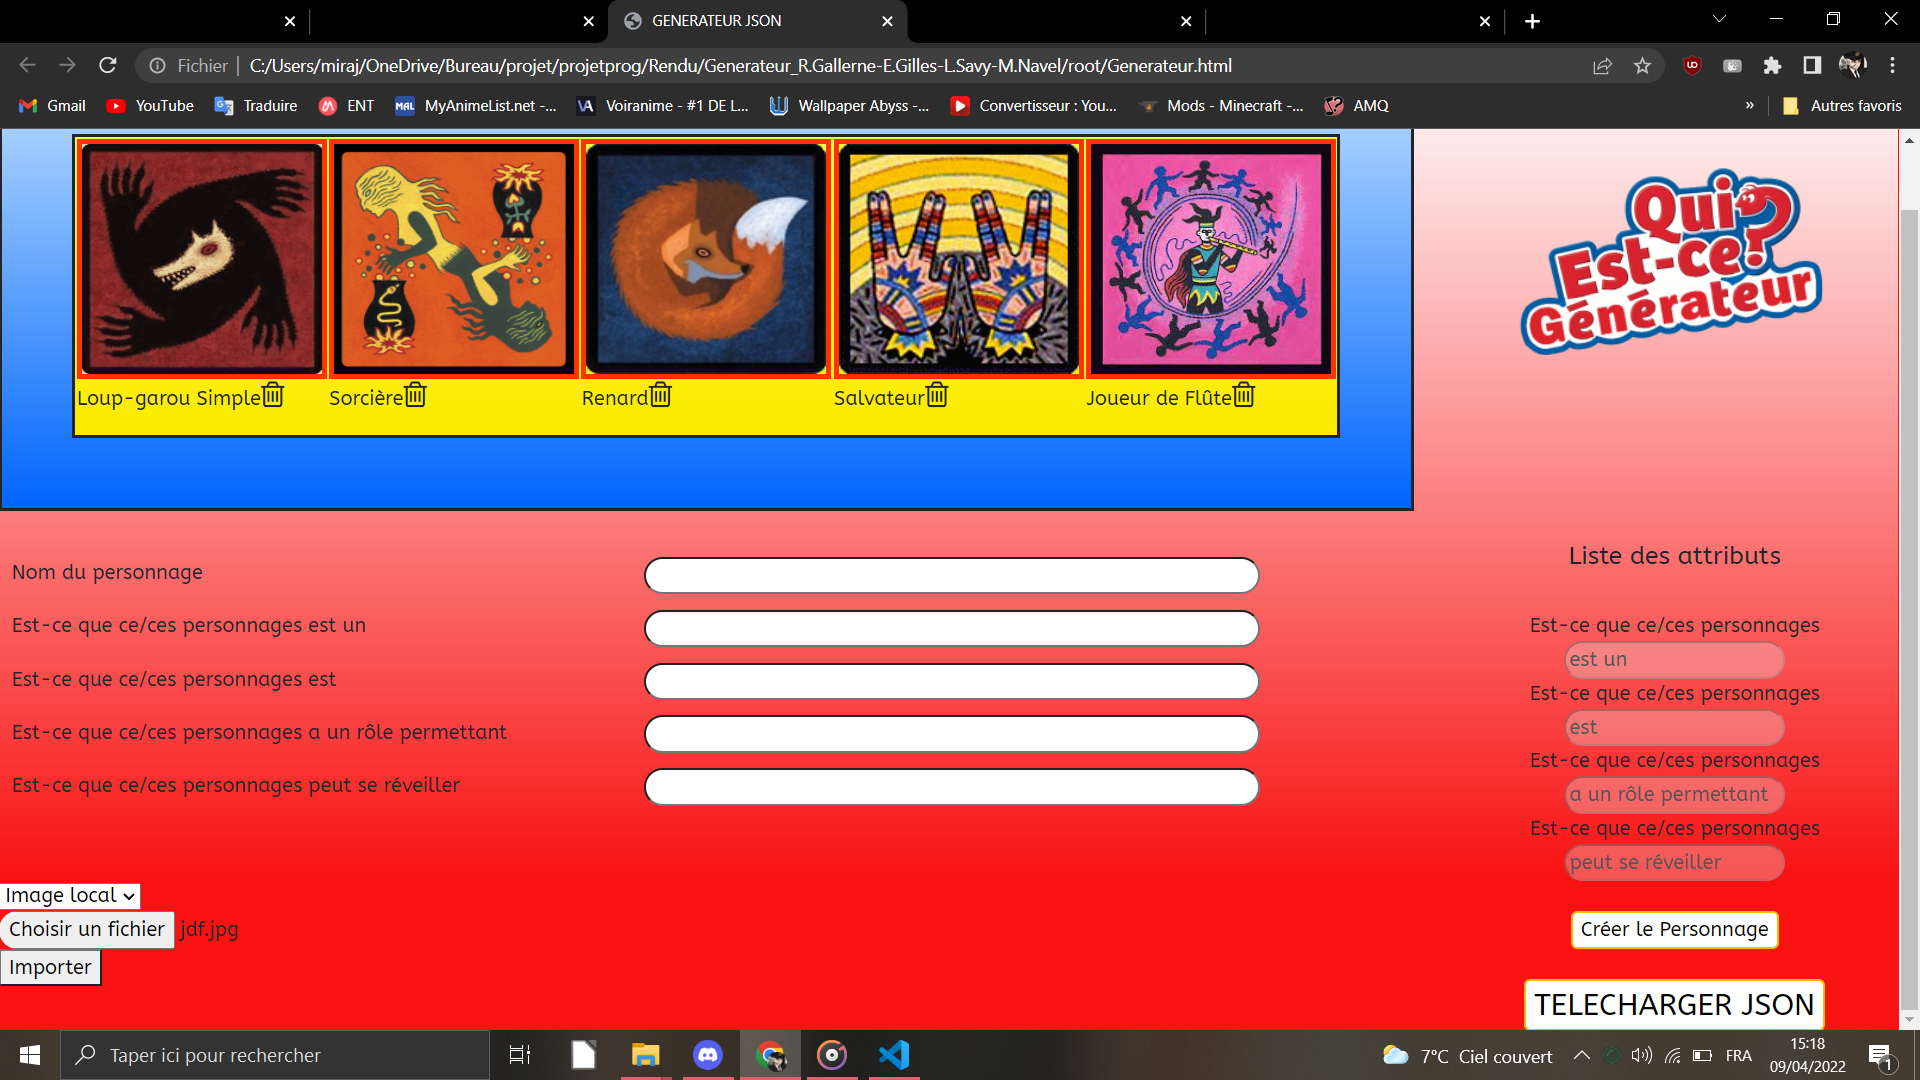
\includegraphics[width=15cm]{images/generateur.png}
            \caption{Rendu du générateur}
        \end{figure}
        
        \subsection{Description des formats de données utilisés et résultat}
            L'objectif de ce logiciel et de traiter des données entrées par l'utilisateur afin de rendre à la fin un fichier au format JSON pour qu'il puisse être utilisé sur notre jeu principal \textsf{Qui est-ce?}\\
            \par  Le format JSON est formaté comme décrit dans la Partie 2 : \textsf{Jeu principal} et c'est en fonction de lui que nous avons choisi nos différents formats de données.
            
            \subsubsection{Les personnages}
                Quand l'utilisateur crée un personnage, un objet JavaScript est créé. Celui-ci contient 3 attributs :
                \begin{itemize}
                    \item "\texttt{nom}" : une chaîne de caratère (String),
                    \item "\texttt{image}" : une chaîne de caratère (String) et
                    \item "\texttt{attributs}" : un objet JavaScript indexé par les noms des attributs renseignés par l'utilisateur.
                \end{itemize}
                Les valeurs de ces attributs vont être décrites dans les sous-parties suivantes.\\
                Quand l'utilisateur appuiera sur le bouton \textsc{Créer le Personnage}, l'objet du personnage sera stocké dans un autre objet Javascript indexé par les noms des personnages créés.
            
            \subsubsection{Le nom des personnages}
                Quand l'utilisateur rentrera le nom de son personnage, celui-ci ne sera pas définitif tant que l'utilisateur ne créera pas son personnage. Il en sera de même pour toutes les autres données entrées par l'utilisateur, elles ne seront stockées que quand le personnage sera créé.\\
                Quand le personnage sera créé, le nom va être stocké dans l'attribut "\texttt{nom}" de l'objet JavaScript du personnage qui vient d'être créé.\\
                \par Nous avons également décidé d'afficher dynamiquement les entrées de l'utilisateur comme le \textsf{nom}, les \textsf{attributs} ou les \textsf{valeurs}. Les entrées ne sont pas réellement stockée, nous manipulons seulement le DOM.
            
            \subsubsection{Les images}
                L'utilisateur aura le choix d'importer une image locale ou via un lien URL.\\
                Si l'image est importée via un lien URL, le lien est tout simplement stocké sous forme de chaîne de caractères (String) dans l'attribut "\texttt{image}" de l'objet JavaScript du personnage qui vient d'être créé.
            
            \subsubsection{Les attributs}
                Quand l'utilisateur éditera son premier personnage, il devra renseigner tous les attributs qu'il souhaitera donner aux personnages. Tous les personnages auront les même attributs, seules leurs valeurs diffèreront.
                Quand ce premier personnage sera validé, les attributs ne seront plus modifiables et stockés dans l'attribut "\texttt{attributs}". Chaque attribut rentré par l'utilisateur deviendra une clé de l'objet JavaScript "\texttt{attributs}" de chaque personnage, les valeurs associées à chaque attribut seront celles renseignées dans les zones de saisie des valeurs comme expliqué après.
            
            \subsubsection{Les valeurs}
                A chaque personnage que l'utilisateur créera, il devra lui renseigner des valeurs pour chaque attribut (celles-ci peuvent être vides mais chaque combinaison de valeurs doit être unique). Ces valeurs seront stockées dans l'attribut "\texttt{attributs}" du personnage qui vient d'être créé. Chaque clé de l'attribut "\texttt{attributs}" sera associé à la valeur corresponde renseignée par l'utilisateur.
        
        \subsection{Les différentes interactions possibles}
            Pour créer une grille de personnages, il faudra que l'utilisateur crée chaque personnage un à un. Pour créer un personnage, il pourra soit commencer par importer une image ou directement rentrer les données du personnage qu'il souhaite créer et importer l'image après ou durant la création du personnage.\\
            
            \subsubsection{Importer une image}
            \begin{figure}[h]
                \centering 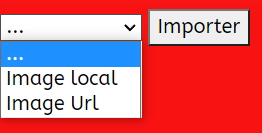
\includegraphics[width=7cm]{images/importer.png}
                \caption{Choix du mode d'importation d'image}
            \end{figure}
            {\large \textbf{Attention}!} Il est recommandé d'utiliser des images au format carré pour éviter que celles-ci soient compressées.\\
            
            \pagebreak
                {\large Il y a deux façons d'importer des images (cf.\textsc{Figure 8}):}
                \begin{itemize}
                \item \underline{\textsf{Importer une image avec un URL}}\\
                    Quand l'utilisateur choisira cette option, une zone d'entrée de texte apparaîtra juste en-dessous. Il suffira à l'utilisateur de saisir l'URL de l'image désirée et de cliquer sur importer pour que l'image s'affiche (cf. \textsc{Figure 9}). \textit{Il sera nécessaire d'avoir accès à Internet pour voir l'image.}\\
                \end{itemize}
                \begin{figure}[h]
                        \centering 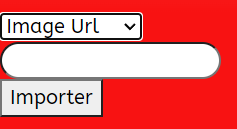
\includegraphics[width=7cm]{images/importURL.png}
                        \caption{Importer une image avec un URL}
                \end{figure}
                
                \begin{itemize}
                \item \underline{\textsf{Importer une image locale}}\\
                    Quand l'utilisateur choisira cette option, un bouton apparaîtra et il pourra ainsi sélectionner l'image désirée dans son ordinateur et cliquer sur le bouton importer pour que l'image s'affiche (cf. \textsc{Figure 10}).
                    \textit{Choisir d'utiliser des images locales alourdira le fichier JSON car le lien de chaque image est entièrement recodée en caractères (environ 60000 caractères).}
                \end{itemize}
                \begin{figure}[h]
                    \centering 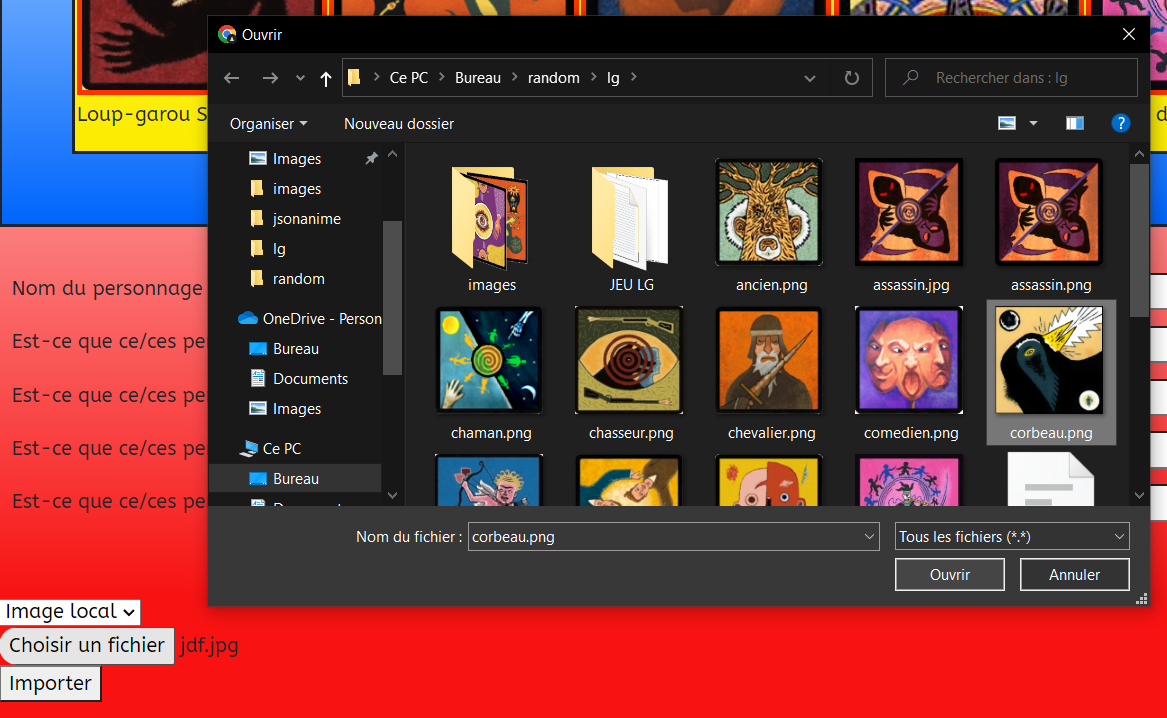
\includegraphics[width=10cm]{images/importLocal.png}
                    \caption{Importer une image locale}
                \end{figure}
                \begin{center}
                    Tant que le personnage n'est pas créé, le bouton Importer restera grisé.
                \end{center}
            \pagebreak
            
            \subsubsection{Créer les attributs}
                Quand l'utilisateur commencera à créer son premier personnage, il devra rentrer la liste \textbf{définitive} des attributs qu'auront tous les personnages dans la zone de saisie à droite de la page (cf. \textsc{Figure 11}). L'utilisateur peut supprimer l'attribut de son choix ou en ajouter jusqu'à 15 tant qu'il est en train de créer son premier personnage. Quand celui-ci sera validé, l'utilisateur ne pourra plus du tout toucher à cette liste. Il ne doit pas y avoir d'attribut \textbf{vide}!\\
                \begin{figure}[h]
                    \centering 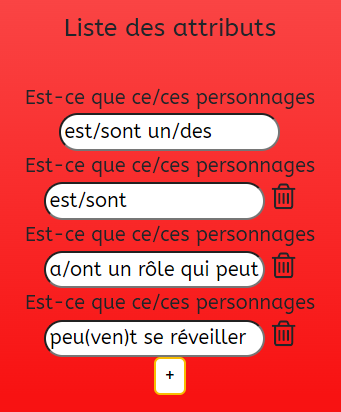
\includegraphics[width=5cm]{images/exempleAttributs_creation.PNG} 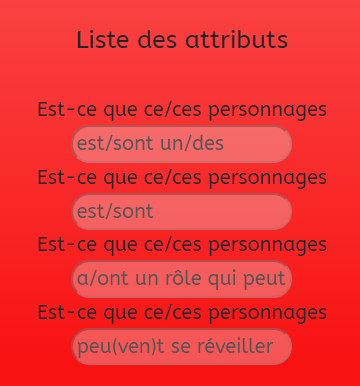
\includegraphics[width=5cm]{images/exempleAttributs_fige.PNG}
                    \caption{Liste d'attributs avant et après création}
                \end{figure}\\
                \par Il est conseillé à l'utilisateur de créer des attributs cohérents avec le format de questions du jeu (notamment de considérer le pluriel au vu du mode Double Personnage).\\
                Les questions en mode \textsf{Normal} commencent toujours par \textit{Est-ce que le personnage} (cf. \textsc{Figure 12}). Pour que la phrase est un sens, l'utilisateur doit rentrer un attribut commençant par un verbe conjugué.\\
                \begin{figure}[h]
                    \centering 
\includegraphics[width=12cm]{images/exempleQuestionNormal.png}
                    \caption{Exemple d'un question en mode Normal}
                \end{figure}
                \par Quand le mode \textsf{Double Personnage} est sélectionné, la question commence toujours par \textit{Est-ce que} suivi de \textsl{aucun des personnages}, \textsl{au moins un des personnages} ou \textsl{les deux personnages} (cf. \textsc{Figure 13}). Pour que la phrase est un sens, l'attribut doit commencer par un verbe conjugué prenant en compte le pluriel. Le pluriel n'est pas nécessaire mais conseillé pour se rapprocher au mieux du langage naturel.\\
                \begin{figure}[h]
                    \centering 
\includegraphics[width=12cm]{images/exempleQuestionDouble.png}
                    \caption{Exemple d'un question en mode Double Personnage}
                \end{figure}\\
                
                {\large \textbf{Attention}!} La question ne se finit pas juste après l'attribut mais après la valeur! Il ne faut donc pas créer une question qui oblige que les valeurs d'attributs soit \textit{oui} ou \textit{non} sinon les réponses à ce genre de questions seront peu claires et porteront à confusion (cf. \textsc{Figure 14}).\\
                \begin{figure}[h]
                    \centering 
\includegraphics[width=12cm]{images/exempleQuestionMalFaite.png}
                    \caption{Exemple de question mal pensée}
                \end{figure}
            \pagebreak
            
            \subsubsection{Les valeurs d'attributs des personnages (et son nom)}
                Les valeurs d'un personnage sont entrées lors de sa création et ne pourront plus être modifiées après. La zone pour entrer les valeurs se situe juste en-dessous du rendu des images (cf. \textsc{Figure 15}).\\
                \begin{figure}[h]
                    \centering 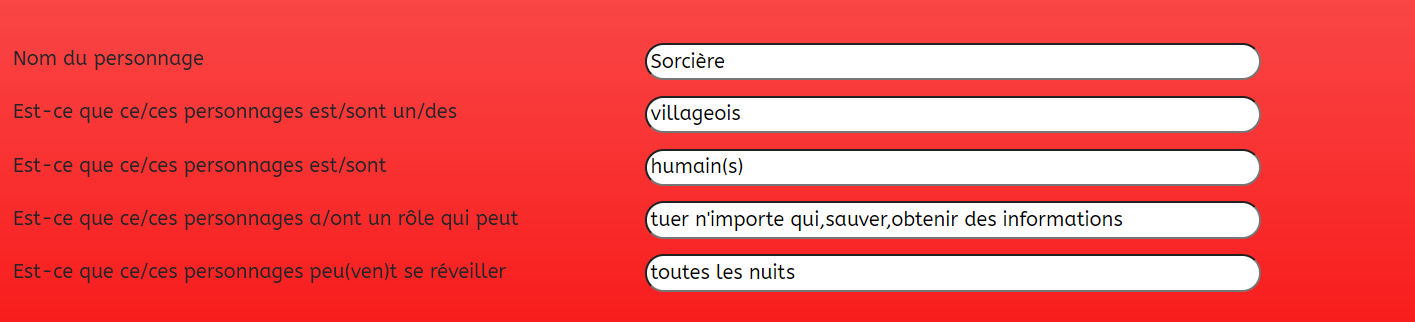
\includegraphics[width=12cm]{images/exempleValeurs.PNG}
                    \caption{Exemple de liste de valeurs}
                \end{figure}
                
                Afin d'aider à la compréhension, le début de la question (\textsf{Est-ce que} + attribut affiché dynamiquement) est indiqué juste devant les zones de saisie.\\
                Quand le nom est rentré par l'utilisateur, il s'affiche dynamiquement sous l'image du personnage en cours d'édition.\\
                Comme vu en \textsc{Figure} ..., l'utilisateur peut rentrer plusieurs valeurs pour un même attribut, celles-ci peuvent contenir des espaces et des apostrophes mais il faut bien faire attention à séparer chaque valeur par une virgule et seulement une virgule (si l'utilisateur rentre un espace juste après il sera pris en compte dans la deuxième valeur d'attribut).
                
            \subsubsection{Valider et supprimer un personnage}
                Quand l'utilisateur sera satisfait de sa grille de personnages, il lui suffira de cliquer sur le bouton "Conversion JSON" et le rendu sous format JSON de la grille se téléchargera et sera stockée dans le dossier Téléchargement de l'utilisateur.
            \pagebreak


    \section{Extension : Mode Double Personnages}
        {\large Pour notre projet, nous avons décidé d'ajouter le mode \textsf{Double Personnage} en tant qu'extension.}\\
        L'objectif de cette extension est  d'augmenter la difficulté du jeu et d'utiliser la logique des quesions de notre jeu de base afin de voir comment complexifier la façon dont l'utilisateur posera des questions.\\
        
        \subsection{Description de l'extension}
            L'utilisateur, en activant ce mode, devra trouver deux personnages, avec des questions qui sont formés différemment. En effet, comme on peut le voir sur la \textsc{Figure 16} , la forme est très similaire aux questions du jeu de base, mais avec en plus une information pour savoir si "\textsl{au moins un des personnages}", "\textsl{les deux personnages}" ou "\textsl{aucun des personnages}" vérifient la question demandée, tout en utilisant les connecteurs logiques "\textsc{ou}" et "\textsc{et}" du jeu de base.\\
            \begin{figure}[h]
                \centering
                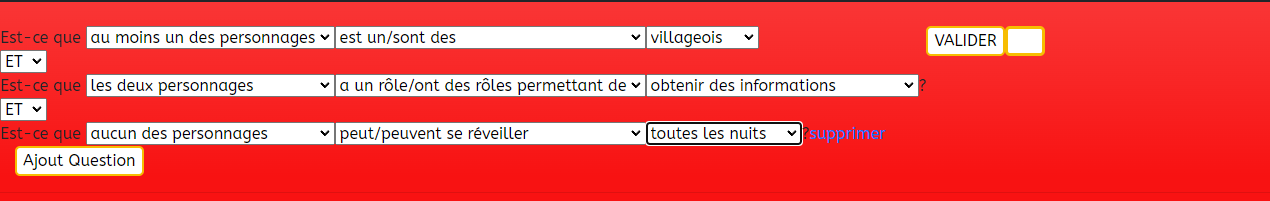
\includegraphics[width=10cm]{images/QuestionExtension.png}
                \caption{Exemple de la formation de questions en mode double personnage}
            \end{figure}
            Lorsque le bouton d'activation du mode \textsf{Double Personnage} est activé, nous avons fait le choix de ne pas pouvoir revenir en arrière lorsque celui-ci est activé. On ne peut donc pas le désactiver (voir \textsc{Figure 17}).\\*
            De plus une petite ligne apparaît pour l'informer du nombre d'essais restant. Quand ce mode est activé, le nombre de tentatives passe de 3 à 6. Nous avons aussi fait le choix de ne pas pouvoir activer le mode \textsf{Facile} car celà prendrait beaucoup plus de temps que ce qu'on nous permet.\\
            
            \begin{figure}[h]
                \centering
                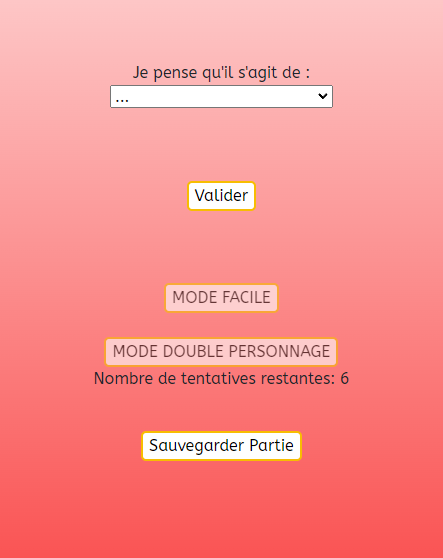
\includegraphics[width=6cm]{images/BoutonModeDoublePersonnage.png}
                \caption{Image des boutons après activation du mode \textsf{Double personnage}}
            \end{figure}
            
            \pagebreak
        
            De plus, quand l'utilisateur fait une tentative et trouve un des deux personnages un message l'informant qu'il a bien trouvé un des deux personnages apparaît (voir \textsc{Figure 18}).\\*
            La condition de victoire étant d'avoir trouvé le deuxième personnage, le message affiché sera comme dans la \textsc{Figure 19}\\
            \begin{figure}[h]
                \centering
                
\includegraphics[width=10cm]{images/DecouverteD'unPersonnage.png}
                \caption{Message lors de la découverte d'un des deux personnages}
            `\end{figure}
            
            \begin{figure}[h]
                \centering
                
\includegraphics[width=10cm]{images/DecouverteDuPersonnageDeux.png}
                \caption{Message lors de la découverte du deuxième personnage}
            \end{figure}
            
        \subsection{Description de la mise en oeuvre de l'extension}
            \subsubsection{Initialisation du mode \textsf{Double personnage}}
                \begin{figure}[h]
                    \centering 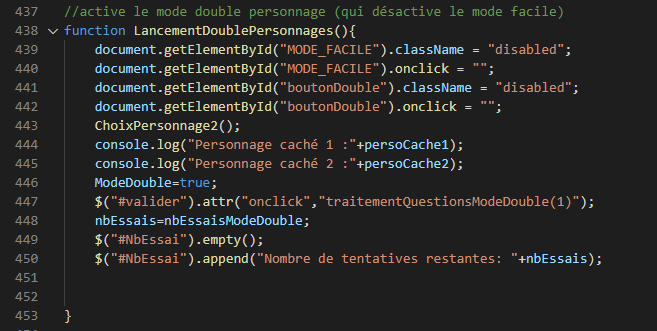
\includegraphics[width=10cm]{images/LancementDoublePersonnage.png}
                    \caption{Extrait du code du lancement du mode}
                \end{figure}
                La fonction \texttt{LancementDoublePersonnages()} (voir Figure 20) va faire principalement des modifications dans le DOM. Elle va dans un premier temps désactiver les boutons \textsc{Double Personnage} et \textsc{Mode Facile} présent sur la page comme expliqué précedemment, puis elle va exécuter la fonction \texttt{ChoixPersonnage2()} qui se charge de donner un personnage aléatoire pour le deuxième personnage.\\*
                \texttt{LancementDoublePersonnages()} actualise aussi le nombre d'essais de 3 à 6 et ajoute une variable global booléenne \texttt{ModeDouble} qui permet de savoir à n'importe quel moment dans notre programme si ce mode est activé.\\*
                Et enfin, cette fonction change l'événement \texttt{onclick()} du bouton de validation d'une question de la manière dont on doit traiter une question dans ce mode.
                
            \subsubsection{Création des Questions}
                Dans ce mode, les questions sont un peu différentes, ce qui nous oblige à modifier le DOM pour avoir la bonne formulation pour la première question affichée, et pour les questions qui seront ajoutées à la suite comme dans le jeu de base.\\
                Pour celà, nous avons le code en \textsc{Figure 21} et \textsc{22} qui font respectivement la création de la première question et la liste des attributs possibles comme dans le jeu de base avec, en plus, la liste contenant "\textsl{au moins un des personnages}", "\textsl{les deux personnages}" et "\textsl{aucun des personnages}" pour avoir la base dans le HTML.\\*
                Enfin, les fonctions d'ajout et de suppression de questions qui sont très similaire à celles du jeu de base. Dans la fontion d'ajout de question, nous avons ajouté une variable global \texttt{firstTime} afin de pouvoir remettre à zero le compteur de questions du programme pour pouvoir indexer correctements les questions. La fonction de suppression quant à elle supprime la division où se trouve la question, diminue le compteur de questions et actualise l'événement \texttt{onclick()} du bouton \textsc{Valider}.
                \begin{figure}[h]
                    \centering                    \includegraphics[width=15cm]{images/ConstructionPremièreQuestion.png}
                    \caption{Extrait du code de la création de la première question de la page}
                    \vspace{0.5cm} 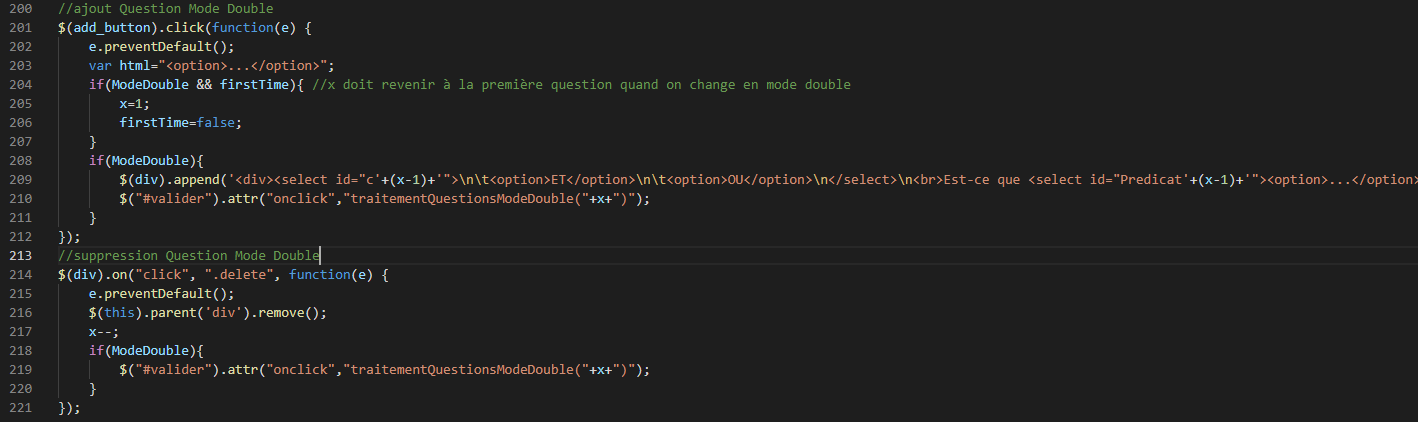
\includegraphics[width=15cm]{images/Ajout&SuppressionQuestionModeDouble.png}
                    \caption{Extrait du code de l'ajout et suppression de question}
                \end{figure}
                
            \subsubsection{Traitement des questions}
                La fonction de traitement est aussi légèrement différent du jeu de base, car il faut traduire "\textsl{au moins un des personnages}", "\textsl{les deux personnages}" et "\textsl{aucun des personnages}" en logique.\\
                Dans un premier temps, nous avons regardé comment traiter UNE question en mode \textsf{Double Personnage}. Ceci est fait par la fonction \texttt{TraitementUneQuestionModeDouble()} (voir \textsc{Figure 23 }l.437).\\
                Finalement, le traitement d'une question c'est simplement le traitement d'une question utilisant la même fonctionnalité que le jeu de base (on l'appelera traitement simple), mais avec une différence c'est que l'on a deux personnages, donc on différencie les cas pour savoir quel connecteur logique utilisé ("\textsc{et}" si le joueur a choisi "\textsl{les deux personnages}", "\textsc{ou}" si le joueur a choisi "\textsl{au moins un des personnages}" et "\textsc{non(ou)}" si le joueur a choisi "\textsl{aucun des personnages personnages}") et ensuite on applique ce connecteur logique sur le retour booléen du traitement simple sur le premier personnage avec le retour booléen du traitement simple du deuxième personnage.\\
                Cette fonction prend donc en paramètre le \textsf{Prédicat} selectionné (sous entendu "\textsl{au moins un des personnages}", "\textsl{les deux personnages}" ou "\textsl{aucun des personnages}"), l'attribut sélectionné et la valeur selectionnée, et rend en fonction de ces paramètres une valeur booléen \textsc{Vrai} ou \textsc{Faux}.
                
                \pagebreak
                
                Enfin, pour plusieurs questions effectuées par la fonction traitementQuestionsModeDouble (voir Figure 23  l.405 - 434), il suffit de prendre une valeur tampon que l'on initialise au retour booléen de la première question indexée par 0, et ensuite, en fonction du connecteur "\textsc{et}" ou "\textsc{ou}", on applique ce connecteur binaire entre le retour booléen "tampon" et la valeur booléenne de la question courante.\\
                La fonction prend en entrée le nombre de questions dans la page (d'où le besoin d'actualiser le nombre de questions) et elle renvoie un valeur booléenne.
            \begin{figure}[h]
                \centering
                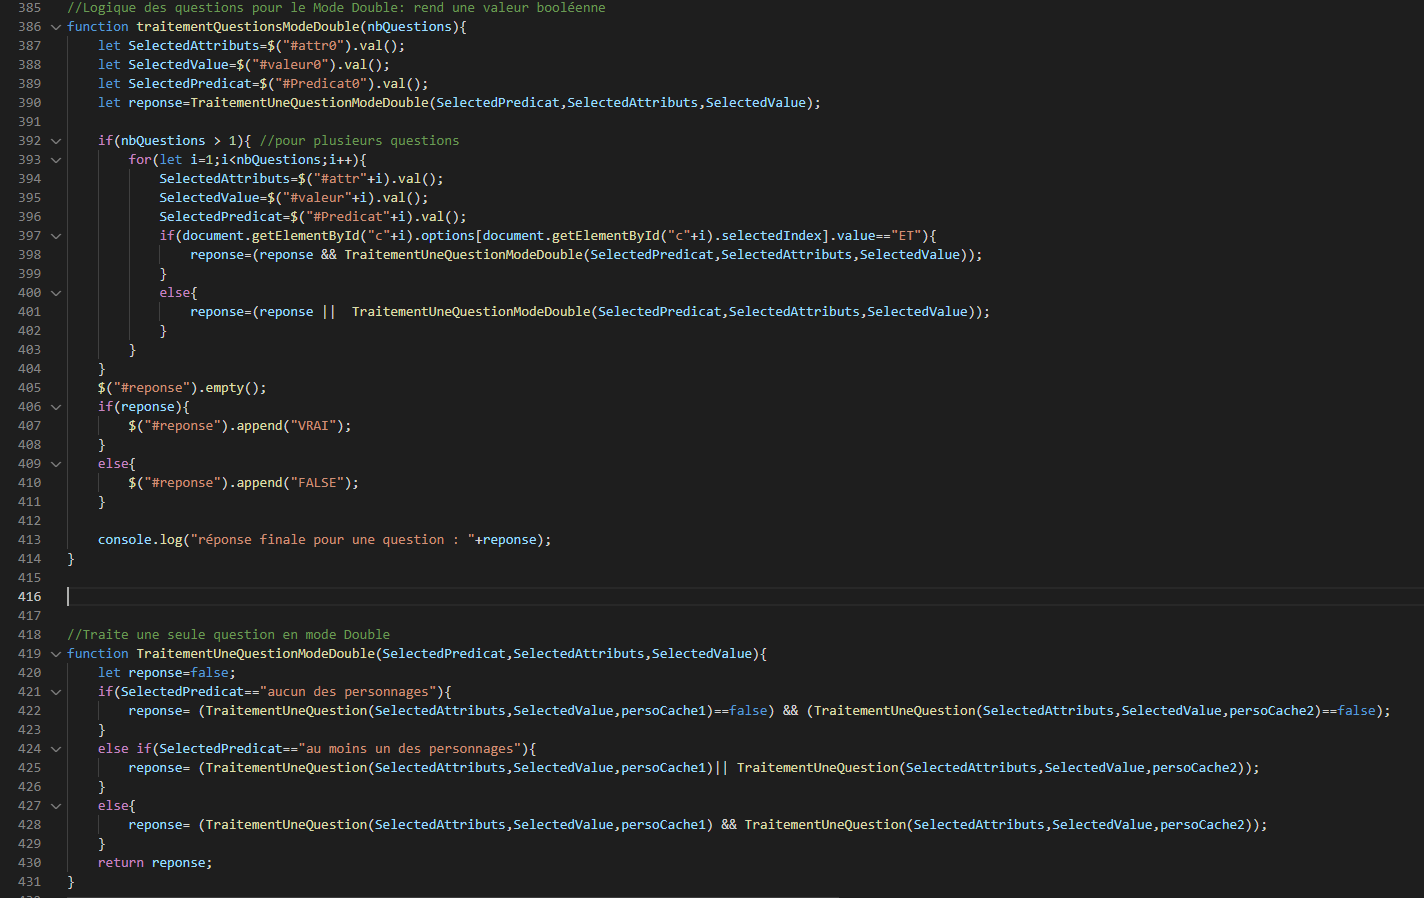
\includegraphics[width=15cm]{images/TraitementQuestionModeDouble.png}
                \caption{Extrait du code du traitement de plusieurs questions}
            \end{figure}
            
    \pagebreak
            
    \section{Conclusion}
        \subsection{Problèmes rencontrés}
            Nous avons eu des problèmes liés au développement du projet de programmation :
            \begin{itemize}
                \item Le premier problème qui s'est présenté à nous très vite a été la gestion et récupération du fichier JSON que nous avions prévu de gérer dynamiquement. Nous avons finalement choisi de le récupérer dès le début dans une variable globale.
                \item Lors de la suppression des questions, nos indices se décalaient systématiquement, nous avons donc du réécrire entièrement cette fonction.
                \item Pour la sauvegarde de la partie de jeu, nous avons voulu utiliser les cookies de JavaScript mais nous avons changé pour les LocalStorage pour une facilité de développement. Le stockage local est majoritairement utilisé pour les applications clients et n'ont pas de dates d'expiration comparés aux cookies.
                \item Enfin, nous avons malgré nous passé beaucoup de temps sur de l'HTML et du CSS afin de rendre notre application la plus agréable possible à utiliser. 
            \end{itemize}
        \subsection{Bilan}
            \par Ce projet nous a permis d'acquérir et de renforcer des notions en développement Web que nous avons vu en cours  et précisement en JavaScript et en Jquery pour la réalisation d'une application Web d'un jeu Qui est-ce?.\\
            \par Cela nous a aussi donner la possibilité de modéliser des maquettes de la page de jeu et de création de JSON que nous devions réaliser pour permettre de disposer facilement les différents éléments graphiques et les emplcaments des menus et ainsi faciliter la réalisation de l'application Web.\\
            \par Au niveau de la gestion de projet, cela nous a donner l'occasion de travailler en groupe sur un projet avec un but bien défini et de nous répartir sur les différentes tâches à réaliser.
\end{document}